\title{Fourier from the ground up}

\newcommand{\Z}{\mathbf{Z}}
\newcommand{\Q}{\mathbf{Q}}
\newcommand{\R}{\mathbf{R}}
\newcommand{\C}{\mathbf{C}}
\newcommand{\T}{\mathbf{T}}
\newcommand{\PP}{\mathcal{P}}
\newcommand{\ud}{\mathrm{d}}
\newcommand{\ds}{\displaystyle}
\newcommand{\DFT}{\mathtt{DFT}}
\newcommand{\IDFT}{\mathtt{IDFT}}



\clearpage
\section{Prerequisites}

We assume basic knowledge of real and complex numbers, calculus, and algebra.
None of the following formulas should be any surprise to you:

$$e^{a + bi}=e^a\left(\cos b+i\sin b\right)$$

%$$f'(x)=\lim_{h\to 0}\frac{f(x+h)-f(x)}h$$

$$ f(x)=
\sum_{n\ge0}\frac{1}{n!}f^{(n)}(0)x^n$$
%f(0) + f'(0)x + \frac{1}{2} f''(0)x^2 + \cdots +
%\frac{1}{n!}f^{(n)}(0)x^n+\cdots $$

$$ \int_a^b f'(x)\ud x = f(b) - f(a) $$

$$ \frac{\ud}{\ud x}\int_a^x f(t)\ud t = f(x) $$

\vfill

We denote by~$\T$ the quotient of the additive group~$\R$ by the
subgroup~$2\pi\Z$.  Thus, functions~$f:\R\to\C$ that are~$2\pi$-periodic can
be understood as functions~$f:\T\to\C$, and their integral over one period is
denoted indistinctly as
$$
\int_\T f
\quad = \quad
\int_\T f(\theta)\,\ud\theta
\quad = \quad
\int_0^{2\pi} f(\theta)\,\ud\theta
\quad = \quad
\int_{-\pi}^{\pi} f(\theta)\,\ud\theta
$$

Notice that the elements of~$\T$ can bijectively identified by numbers
in~$[0,2\pi)$, but the topological spaces~$\T$ and~$[0,2\pi)$ are different.
For example, the function~$\cos\frac\theta2$ is continuous on~$[0,2\pi)$
but discontinuous on~$\T$, while the function~$\sin\frac\theta2$ is
continuous on both spaces, bot only differentiable on~$[0,2\pi)$.

\includegraphics{fsincos1.png}
%SCRIPT cat <<END | gnuplot > fsincos1.png
%SCRIPT set term pngcairo crop size 720,300
%SCRIPT set samples 1000
%SCRIPT set xtics 1
%SCRIPT fmod(x,y)=x-y*floor(x/y)
%SCRIPT plot [-3:9] [-2:3] cos(fmod(x,2*pi)/2),sin(fmod(x,2*pi)/2)
%SCRIPT END

\vfill

\clearpage
\section{The algebra of trigonometric polynomials}


\begin{definition}
A~\emph{trigonometric polynomial} is an expression of the form
$$
	f(\theta)=\sum_{n\in\Z} F_n e^{in\theta}
$$
where all the coefficients~$F_n\in\C$ are zero except, maybe, a finite
number of them.  The set of all trigonometric polynomials is denoted
by~$\PP$.
\end{definition}

There are two ways to interpret a trigonometric polynomial: as a
function~$\Z\to\C$ defined by~$n\mapsto F_n$, or as a function~$\R\to\C$
defined by~$\theta\mapsto f(\theta)$.
Most of Fourier analysis deals with
the duality between these two interpretations.
There is a third interpretation, as finite Laurent series~$f(z)$ evaluated on
the unit circle~$z=e^{i\theta}$, but it is of minor interest for the present
course.

Let us introduce some {\bf common language}.
A trigonometric polynomial is usually called a~\emph{signal}.  The
indices~$n$ are called the~\emph{frequencies} and the coefficient~$F_n$
is called the~\emph{amplitude of~$f$~at the frequency~$n$}.  The
mapping~$n\mapsto\left|F_n\right|^2$ is called the~\emph{power
spectrum} of the signal~$f$.  Building the signal from its amplitudes
is called is called~\emph{synthesis}, and extracting the amplitudes
from a signal is called~\emph{analysis}.

The monomial~$e^{in\theta}$ is called a~\emph{pure wave of frequency~$n$}.
Thus, synthesis consists in creating a signal as a linear combination of pure
waves, and analysis consists in recovering the coefficients of this linear
combination.  Using this language, we say that harmonic analysis consists in
studying the duality between signals~$f(\theta)$ and their spectra~$F_n$; how
do the operations on signals correspond to operations on their spectra, and
vice-versa.

%{\bf Proposition (algebraic properties of~$\PP$).}
%The space~$\PP$ is a vector space over~$\C$ and also an algebra.  The
%(algebraic) inner product on~$\PP$
%$$
%\left\langle f,g\right\rangle_a=\sum_{n\in\Z}f_n\bar{g_n}
%$$ is hermitian, and with the associated
%norm~$\|f\|_a=\sqrt{\left\langle f,f\right\rangle_a}$, the set of
%monomials~$e^{in\theta}$ is an orthonormal basis of~$\PP$.
%This vector space is neither finite-dimensional nor complete with this norm.


\begin{proposition}\label{prp:elementary}
(Elementary properties)
The following properties hold:
\begin{enumerate}
	\item If~$f\in\PP$ then~$f(\theta)$ is a
		function~$\R\to\C$ which is~$2\pi$-periodic
		and~$\mathcal{C}^\infty$.
	\item If~$f\in\PP$ then~$F_n$ is a function~$\Z\to\C$ of finite
		support.
	\item The set~$\PP$ is a vector space over~$\C$.
	\item If~$h=\lambda f+\mu g$ then~$H_n=\lambda F_n+\mu G_n$.
	\item The set~$\PP$ is an algebra (thus, closed by
		pointwise product~$f(\theta)g(\theta)$)
\end{enumerate}
\end{proposition}

\begin{proof}
(1) Each monomial~$e^{in\theta}$ is~$\mathcal{C}^\infty$
	and~$2\pi$-periodic, and~$f$ is a finite linear
	combination of such monomials, so it is
	also~$\mathcal{C}^\infty$ and~$2\pi$-periodic.
(2) This is a rewriting of the defintion of~$\PP$.
(3,4) This result is immediate by linearity of finite sums.
(5) The product of two finite sums is still a finite sum.
\end{proof}

The point~(3) of this proposition is of fundamental importance.  In a more
general context, it is called the \emph{superposition principle}.  Although it
is algebraically trivial, it may be non-intuitive when using the language of
signal processing: when computing the sum of two signals, their amplitudes at
each frequency add up separately. \emph{There can be no destructive
interference between different frequencies.}

\begin{proposition}(Symmetry properties)
\begin{enumerate}
	\item $f$ even $\iff$ $F$ even
	\item $f$ real $\iff$ $F$ hermitian
	\item $f$ real and even $\iff$ $F$ real and even
	\item $f$ real and odd $\iff$ $F$ pure imaginary and odd
\end{enumerate}
\end{proposition}

\begin{definition}(Examples of trigonometric polynomials)
	Here we show several examples of trigonometric polynomials.  They are
	all very important and will be used later.  For each case we specify
	the values of their non-zero amplitudes.
\begin{enumerate}
	\item The pure waves: $e_n(\theta)=e^{in\theta}$
		$\qquad F_n=1$
	\item The pure waves with a phase offset:
		$e_{n,\psi}(\theta)=e^{in(\theta+\psi)}$
		$\qquad F_n=e^{in\psi}$
	\item The cosine waves:
		$\cos(n\theta)=\displaystyle\frac{e^{in\theta}+e^{in\theta}}{2}$
		$\qquad F_n=F_{-n}=\frac{1}{2}$
	\item The sine waves:
		$\sin(n\theta)=\displaystyle\frac{e^{in\theta}-e^{in\theta}}{2i}$
		$\qquad F_n=-F_{-n}=\frac{1}{2i}$
	\item The Dirichlet kernel:
		$\mathcal{D}_N(\theta)=\displaystyle\sum_{n=-N}^Ne^{in\theta}$
		$\qquad F_n=1\ ,\ |n|\le N$
	\item The Fejér kernel:
		$\mathcal{K}_N(\theta)
		=\displaystyle\frac{1}{N}\sum_{n=0}^{N-1}\mathcal{D}_n(\theta)
		$%=\sum_{n=-N}^N\frac{N-|n|}{N}e^{in\theta}$
		$\qquad F_n=\frac{N-|n|}{N}\ ,\ |n|\le N$
	\item The Gibbs kernel:
		$\mathcal{G}_N(\theta)
		=\displaystyle\sum_{n=1}^{N}\frac{\sin n\theta}{n}$
	\item The odd sampling kernel:
		$\mathcal{Z}_{2N+1}(\theta)=\frac{1}{2N+1}\mathcal{D}_N(\theta)$
	\item The even sampling kernel:
		$\mathcal{Z}_{2N}(\theta)=\frac{\mathcal{D}_N(\theta)+\cos\frac{N\theta}{2}}{2N}$
\end{enumerate}
\end{definition}


When interpreting a trigonometric polynomial as a~$2\pi$-periodic
function~$\R\to\C$, it helps to plot it as a closed curve in the complex
plane.  The monomials~$e^{in\theta}$ for~$n\neq 0$ all correspond to the unit
circle traversed~$n$ times, clockwise for~$n<0$, anticlockwise for~$n>0$.

\begin{tabular}{ccccccc}
	$e^{-3i\theta}$ &
	$e^{-2i\theta}$ &
	$e^{-i\theta}$ &
	$e^{0i\theta}$ &
	$e^{i\theta}$ &
	$e^{2i\theta}$ &
	$e^{3i\theta}$ \\
	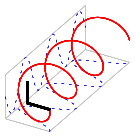
\includegraphics{monomial-3.png} &
	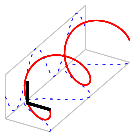
\includegraphics{monomial-2.png} &
	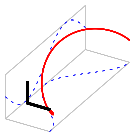
\includegraphics{monomial-1.png} &
	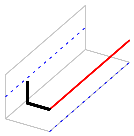
\includegraphics{monomial+0.png} &
	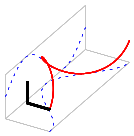
\includegraphics{monomial+1.png} &
	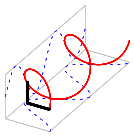
\includegraphics{monomial+2.png} &
	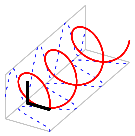
\includegraphics{monomial+3.png} \\
	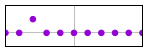
\includegraphics{monoal-3.png} &
	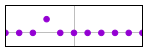
\includegraphics{monoal-2.png} &
	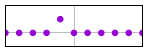
\includegraphics{monoal-1.png} &
	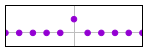
\includegraphics{monoal+0.png} &
	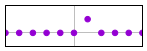
\includegraphics{monoal+1.png} &
	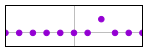
\includegraphics{monoal+2.png} &
	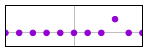
\includegraphics{monoal+3.png} \\
\end{tabular}
%SCRIPT cat <<END >monomial.g
%SCRIPT set term pngcairo crop size 160,160
%SCRIPT unset key; unset border; unset xtics; unset ytics; unset ztics
%SCRIPT set samples 1000; set parametric; set view equal xyz
%SCRIPT set margins at screen 0, at screen 1, at screen 0, at screen 1
%SCRIPT splot [0:2*pi] [-1:1] [-1:1] \
%SCRIPT 	-1,u,-1              lw 0 lc rgb "gray"                  ,\
%SCRIPT 	-1,u,+1              lw 0 lc rgb "gray"                  ,\
%SCRIPT 	+1,u,-1              lw 0 lc rgb "gray"                  ,\
%SCRIPT 	(u-pi)/pi,0,-1       lw 0 lc rgb "gray"                  ,\
%SCRIPT 	(u-pi)/pi,2*pi,-1    lw 0 lc rgb "gray"                  ,\
%SCRIPT 	-1,0,(u-pi)/pi       lw 0 lc rgb "gray"                  ,\
%SCRIPT 	-1,2*pi,(u-pi)/pi    lw 0 lc rgb "gray"                  ,\
%SCRIPT 	cos(f*u),u,-1        lw 0 lc rgb "blue" dashtype '- '    ,\
%SCRIPT 	-1,u,sin(f*u)        lw 0 lc rgb "blue" dashtype '- '    ,\
%SCRIPT 	cos(f*u),u,sin(f*u)  lw 1 lc rgb "red"                   ,\
%SCRIPT 	u/(2*pi),0,0         lw 2 lc rgb "black"                 ,\
%SCRIPT 	0,0,u/(2*pi)         lw 2 lc rgb "black"
%SCRIPT END
%SCRIPT gnuplot -e "f=+0" monomial.g > monomial+0.png &
%SCRIPT gnuplot -e "f=+1" monomial.g > monomial+1.png &
%SCRIPT gnuplot -e "f=+2" monomial.g > monomial+2.png &
%SCRIPT gnuplot -e "f=+3" monomial.g > monomial+3.png &
%SCRIPT gnuplot -e "f=-1" monomial.g > monomial-1.png &
%SCRIPT gnuplot -e "f=-2" monomial.g > monomial-2.png &
%SCRIPT gnuplot -e "f=-3" monomial.g > monomial-3.png &
%SCRIPT wait

%SCRIPT cat <<END >mz.g
%SCRIPT set term pngcairo crop size 192,192
%SCRIPT unset key;unset xtics; unset ytics; set size ratio -1
%SCRIPT set zeroaxis lw 1 lc rgb "gray" lt 1
%SCRIPT plot [-5:5] [-1:2] "< cat -" w circles fill solid
%SCRIPT END
%SCRIPT X=`seq -5 5`
%SCRIPT for i in $X; do echo $i $((i==-3)); done |gnuplot mz.g >monoal-3.png &
%SCRIPT for i in $X; do echo $i $((i==-2)); done |gnuplot mz.g >monoal-2.png &
%SCRIPT for i in $X; do echo $i $((i==-1)); done |gnuplot mz.g >monoal-1.png &
%SCRIPT for i in $X; do echo $i $((i==+0)); done |gnuplot mz.g >monoal+0.png &
%SCRIPT for i in $X; do echo $i $((i==+1)); done |gnuplot mz.g >monoal+1.png &
%SCRIPT for i in $X; do echo $i $((i==+2)); done |gnuplot mz.g >monoal+2.png &
%SCRIPT for i in $X; do echo $i $((i==+3)); done |gnuplot mz.g >monoal+3.png &
%SCRIPT wait


\begin{exercice}
	Prove the following properties of the Dirichlet kernel~$\mathcal{D}_N$:
	\begin{enumerate}
		%\item $\ds\mathcal{D}_N(\theta)$
		\item
			It is a real-valued, even function:
			$\ds\mathcal{D}_N(\theta)=1+2\sum_{n=1}^{N}\cos n\theta$
		\item
			It is a periodic generalization of the sinc function:
			$\ds\mathcal{D}_N(\theta)=\frac{\sin\left(N+\frac{1}{2}\right)\theta}{\sin\frac\theta2}$
		\item
			$\ds\mathcal{D}_N(\theta)=\sin N\theta\cot\frac\theta2+\cos N\theta$
		\item
			Value at zero:
			$\ds\mathcal{D}_N(0)=2N+1$
		\item
			Zero values:
			$\ds\mathcal{D}_N\left(\theta\right)=0
			\iff
			\theta=\frac{2\pi k}{2N+1},
			\quad
			k=\pm 1,\ldots,\pm N$
		\item
			The limit as~$N\to\infty$ is zero almost everyhere:
			$\ds 0<|\theta|\le\pi\ \implies\
			\lim_{N\to\infty}\mathcal{D}_N(\theta)=0$
		\item
			The integral does not depend on~$N$:
			$\ds\int_\T\mathcal{D}_N = 2\pi$
		\item
			The $L^2$ norm goes to infinity very fast:
			$\ds\int_\T\left|\mathcal{D}_N\right|^2 =$
		\item
			The $L^1$ norm goes to infinity slowly
			$\ds\int_\T\left|\mathcal{D}_N\right| =c\log N +
			O(1)\qquad\mathrm{as}\ N\to\infty$
		\item
			Convolution by~$\mathcal{D}_N$ gives partial sums:
			%$\ds f\in\mathcal{P}\implies (\mathcal{D}_N*f)(\theta) =
			%\sum_{|n|\le N} F_ne^{in\theta}$
			$\ds f\in\mathcal{P}\implies \mathcal{D}_N*f = \mathcal{S}_N f$
	\end{enumerate}
\end{exercice}

\begin{exercice}
	Prove the following properties of the Féjer kernel~$\mathcal{K}_N$:
	\begin{enumerate}
		\item
			The amplitudes decay linearly until zero:
			$\ds\mathcal{K}_N(\theta)=\sum_{|n|<N}\frac{N-|n|}{N}e^{in\theta}$
		\item
			It generalizes the squared sinc:
%			$\ds\mathcal{K}_N(\theta)=1+2\sum_{n=1}^{N}\cos n\theta$
%		\item
			$\ds\mathcal{K}_N(\theta)=
			\frac{\sin^2N\frac\theta2}{N\sin^2\frac\theta2}$
		\item $\ds\mathcal{K}_N(0)=2N+1$
		\item $\ds\mathcal{K}_N\left(\frac{2\pi k}{2N+1}\right)=0
			\qquad k=\pm 1,\ldots,\pm N$
		\item
			The limit as~$N\to\infty$ is zero almost everyhere:
			$\ds 0<|\theta|\le\pi\implies\lim_{N\to\infty}\mathcal{K}_N(\theta)=0$
		\item $\ds\int_\T\mathcal{D}_N = 2\pi$
		\item $\ds\int_\T\left|\mathcal{D}_N\right|^2 =$
		\item $\ds\int_\T\left|\mathcal{D}_N\right| =c\log N +
			O(1)\qquad\mathrm{as}\ N\to\infty$
		\item $\ds f\in\mathcal{P}\implies (\mathcal{D}_N*f)(\theta) =
			\sum_{|n|\le N} F_ne^{in\theta}$
		\item
			Convolution by~$\mathcal{D}_N$ gives Cesàro sums:
			%$\ds f\in\mathcal{P}\implies (\mathcal{D}_N*f)(\theta) =
			%\sum_{|n|\le N} F_ne^{in\theta}$
			$\ds f\in\mathcal{P}\implies \mathcal{K}_N*f =
			\frac{\mathcal{S}_0f+\cdots+\mathcal{S}_{N-1}f}{N}$
	\end{enumerate}
\end{exercice}

\subsection{Convolution theorems}

Proposition~\ref{prp:elementary}(3) explains how to analyze the pointwise sum
of two signals.  The convolution theorem explains how to analyze their
pointwise product:

\begin{proposition}[First convolution theorem]
	Let~$h(\theta)=f(\theta)g(\theta)$, then
	\[
		\ds H_n
		= \sum_{k\in\Z} F_kG_{n-k}.
		%= \sum_{k\in\Z} f_{n-k}g_k
		\]
\end{proposition}

\begin{proof}
	The proof is a verification, just as for~\ref{prp:elementary}(3), but
	we write it down fully because it is very important.  By definition we
	have
	\[
		h(\theta)=f(\theta)g(\theta)
		=
		\left(\sum_{n\in\Z}F_ne^{in\theta}\right)
		\left(\sum_{m\in\Z}G_me^{in\theta}\right)
	\]
	expanding the product:
	\[
		=
		\sum_{n\in\Z}\sum_{m\in\Z} F_n G_m e^{i(n+m)\theta}
	\]
	change of variable~$m=k-n$ (keeping~$n$ constant)
	\[
		=\sum_{n\in\Z}\sum_{k\in\Z} F_n G_{k-n} e^{ik\theta}
	\]
	reordering
	\[
		=\sum_{k\in\Z}\left(\sum_{n\in\Z} F_n G_{k-n}\right)e^{ik\theta}
	\]
	thus, identifying the coefficients we have
	that~$\ds h_k=\sum_{n\in\Z} F_n G_{k-n}$.
\end{proof}

The sequence~$h_n=\sum_{k\in\Z} F_k G_{n-k}$ is called the~\emph{discrete
convolution} of the sequences~$F_n$ and~$G_n$.  Thus, the first convolution
theorem says that the spectrum of a pointwise product is the convolution of the
spectra.

The second convolution theorem is the dual version of this statement: the
pointwise product of spectra is the spectrum of the convolution.  For that, we
need to define the convolution of two signals:

\begin{definition}[Convolution of two trigonometric polynomials]
	Let~$f,g\in\PP$.  We define the~\emph{periodic convolution} of~$f$
	and~$g$ as
	\[
		(f*g)(\theta)=\int_0^{2\pi}f(t)g(\theta-t)\ud t
	\]
\end{definition}

\begin{proposition}
	The function~$h=f*g$ is well-defined and it belongs to~$\PP$.
	Moreover,~$h_n=2\pi f_n g_n$.
\end{proposition}

\begin{proof}
	The expression that defines~$(f*g)(\theta)$ is an integral of
	a~$C^\infty$ function on a compact domain, so it gives a finite,
	well-defined number.  We can check that~$f*g\in\PP$ by computing the
	integral explicitly:
	\[
		(f*g)(\theta)=\int_0^{2\pi}f(t)g(\theta-t)\ud t
		=
	\]
\end{proof}


\subsection{Norm, product and energy conservation}


\subsection{Degree}


\subsection{Sampling and the DFT}


\subsection{Zero-padding and aliasing}


\subsection{Analytic properties}

The set~$\PP$ of trigonometric polynomials~$\PP$ is like the set~$\Q$ of rational
numbers. They are both easy to define and manipulate, and all the results about
them can be proved by finite arguments.  However, they have the ugly property
of not being complete nor closed under elementary operations.  For example, the
(pointwise) limit of a sequence of elements of~$\PP$ can be a non-smooth, or
even a discontinuous function, that does not belong to~$\PP$.  Even worse, the
absolute value~$|f|$ of a function~$f\in\PP$ is not typically an element
of~$\PP$.  There are several, different completions of the space~$\PP$.  The most
natural completion of~$\PP$ is the Hilbert space~$L^2([0,2\pi])$, that is
obtained using the norm~$\|f\|_2$ defined above.  We will see that using
stricter norms (involving the derivatives of~$f$) we obtain completions that
are smaller spaces (Sobolev spaces).  And we can even obtain larger completions
(periodic distributions) by using topologies that do not come from any norm.


\subsection{Higher dimensions}

\clearpage
\thispagestyle{empty}

A trigonometric polynomial of~$N$ coefficients is an expression of the form
\[
	f(\theta)=\sum_{n=0}^{N-1} f_n e^{in\theta}
\]
An M-sampling is obtained by evaluating~$f$ at the~$M$
points~$\theta_k=\frac{2\pi k}{M}$.
Sampling theory studies the relationship between the vector of
coefficients~$f_n$ and the vector of samples~$f(\theta_k)$, depending on the
values of~$M$ and~$N$.

\bigskip

The ideal case is when \fbox{$N=M$}, or perfect sampling.  In that case there
are as many coefficients as samples, and there is a linear bijection between
them, whose matrix is given by the DFT:
\[
	f(\theta_k)=\sum_{n=0}^{N-1} f_n e^{\frac{2\pi i k n}{N}}
	\qquad
	k=0,\ldots N
\]
This formula says that the IDFT of the vector~$f_n$ is the
vector~$f(\theta_k)$.

\bigskip

When~\fbox{$M>N$} we have more samples than coefficients.  This is called
oversampling, or redundant sampling, or zero-padding, depending on the point of
view:
\[
	f(\theta_k)=\sum_{n=0}^{N-1} f_n e^{\frac{2\pi i k n}{M}}
	+\sum_{n=N}^{M-1} 0\cdot e^{\frac{2\pi i k n}{M}}
	=\sum_{n=0}^{M-1} zp(f_n) e^{\frac{2\pi i k n}{M}}
\]
where~$zp(f_n)$ is the vector~$f_n$ padded by zeros until length~$M$.
This says that the IDFT of the vector~$zp(f_n)$ is the vector~$f(\theta_k)$.


\bigskip

When~\fbox{$M<N$} we have less samples than coefficients.  This is called
undersampling or aliasing.  We can still write the samples as the IDFT of a
vector involving the coefficients:
\[
	f(\theta_k)
	=
	\sum_{n=0}^{N-1} f_n e^{\frac{2\pi i k n}{M}}
	=
	\sum_{n=0}^{N-1} f_n e^{\frac{2\pi i k (n\% M)}{M}}
\]
where we have performed the euclidean division of~$n$ by~$M$, that
gives~$n=qM+(n\% M)$, and the term containing~$qM$ disappears because the
exponential is~$2\pi$-periodic.  Now, several indices~$n$ may have the same
residue modulo~$M$, and we can group them:
\[
	f(\theta_k)
	=
	\sum_{n=0}^{M-1}\left(\sum_{(n\%M)=m}f_n\right) e^{\frac{2\pi i k m}{M}}
	=
	\sum_{m=0}^{M-1} \mathrm{alias}(f_n) e^{\frac{2\pi i k m}{M}}
\]
so the samples~$f(\theta_k)$ are, as always the IDFT of the
coefficients~$\mathrm{alias}(f_n)$.

\bigskip

{\bf Note:}
The choice of interval for the indices $n\in\{0,\ldots,N-1\}$ may appear
strange, the usual choice
being~$n\in\left\{-\frac{N}{2},\ldots,\frac{N}{2}-1\right\}$.
But we can actually take an arbitrary interval~$I_N\subset\Z$, as long as our
euclidean residue is defined to be inside:~$p\% N\in I_N$.  With this notation,
the formulas above become

\clearpage

This is a trigonometric polynomial of~$N$ coefficients:
\[
	F(\theta)=\sum_{n\in I_N}f_n e^{in\theta}
\]


And those are~$M$ samples:
\[
	\theta_k=\frac{2\pi k}{M} \qquad k=0,\ldots,M
\]

Sampling theory studies the relationship between the vectors~$(f_n)\in\C^N$
and~\mbox{$(F(\theta_k))\in\C^M$}.

\bigskip

The case \fbox{$M=N$} is called ideal sampling.  The relationship is a linear
bijection between samples and coefficients that is, by definition, the~$\DFT$.
\[
	F(\theta_k)=\sum_{n\in I_M}f_ne^{\frac{2\pi ink}{M}}
\]
We have~$F(\theta_k) = \IDFT(f_n)$ (this is our definition of $\IDFT$).

\fbox{$M>N$} oversampling or zero-padding:
\[
	F(\theta_k)
	=
	\sum_{n\in I_N}f_ne^{\frac{2\pi ink}{M}}
	+
	\sum_{n\in I_M\setminus I_N} 0\cdot e^{\frac{2\pi ink}{M}}
	=
	\sum_{m\in I_M}zp(f)_me^{\frac{2\pi imk}{M}}
\]
We have~$F(\theta_k) = \IDFT(zp(f)_m)$, where
\[
	zp(f)_m = \begin{cases}
		f_m & \mathrm{if}\ m\in I_N \\
		0 & \mathrm{if}\ m\in I_M\setminus I_N \\
	\end{cases}
\]

\fbox{$M<N$} undersampling or aliasing:
\[
	F(\theta_k)
	=
	\sum_{n\in I_N}f_ne^{\frac{2\pi ink}{M}}
	=
	\sum_{n\in I_N}f_ne^{\frac{2\pi i(n\% M)k}{M}}
	=
	\sum_{m\in I_M}\left(\sum_{(n\%M)=m}f_n\right)e^{\frac{2\pi imk}{M}}
\]
We still have~$F(\theta_k)=\IDFT(alias(f)_m)$, where
\[
	alias(f)_m=\sum_{(n\ \mathrm{mod}_I\  M)=m} f_n
\]


% vim:set tw=77 filetype=tex spell spelllang=en sw=2 ts=2:
